\lab{Sparse Grids}{SpGrid}
\label{lab:spgrid}

\objective{Introduce Sparse Grids.}

At first inspection, our world appears to be nice and continuous.  However, this only works on a macroscopic level.  As we zoom in on matter, we find that it is made of discrete atoms with much empty space between.  Computers likewise work in discrete space.  You have already seen many examples of this.  Consider plotting the function $y=x^2$, such as in Figure \ref{fig:x_squared}.  To do this we take an array of discrete points of $x$ and $y$ values, which are then joined linearly.  As you either zoom in on the function or decrease the number of plotting points, you can see the discrete nature of even this simple function. 

\begin{figure}
\begin{subfigure}{.5\textwidth}
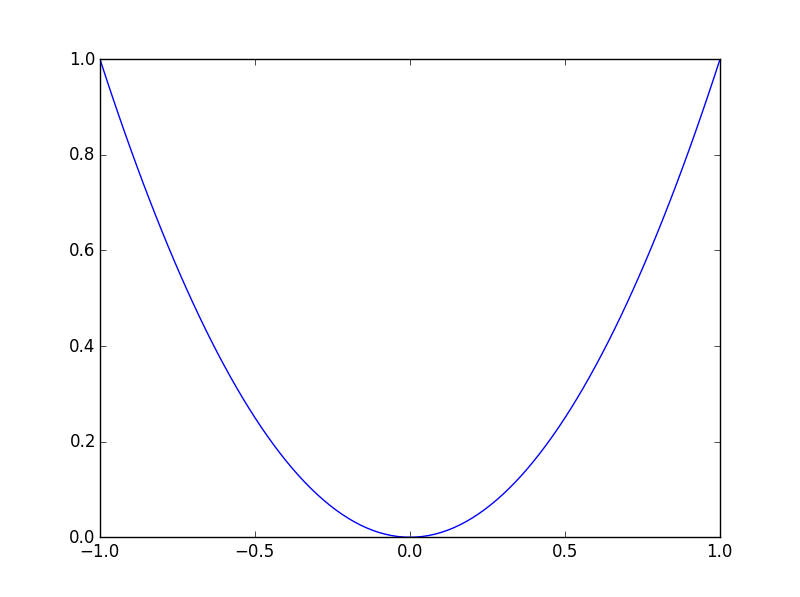
\includegraphics[width=\textwidth]{x2.png}
\end{subfigure}
\begin{subfigure}{.5\textwidth}
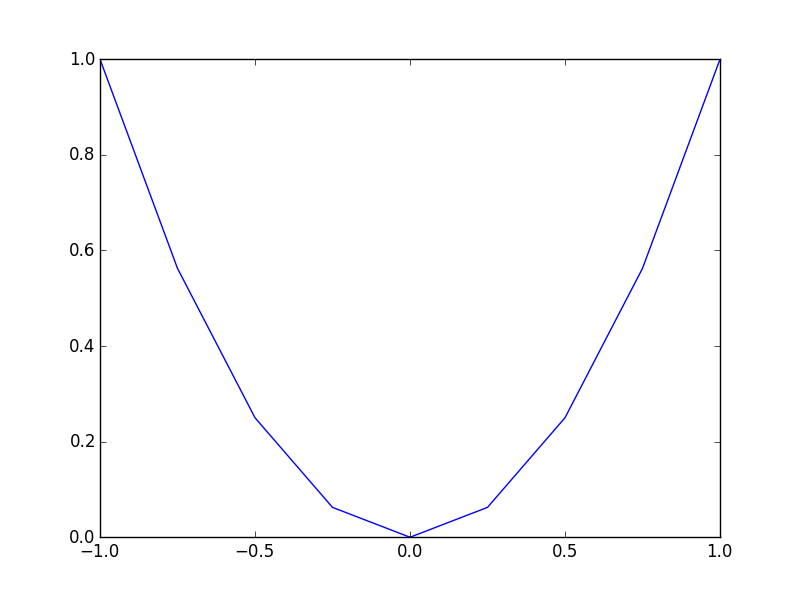
\includegraphics[width=\textwidth]{x2a.png}
\end{subfigure}
\caption{Plots of the function $y=x^2$ using $31$ points and $9$ points, respectively.}
\label{fig:x_squared}
\end{figure}

\section*{First Section}

Say things.

\begin{problem}
Write problems.
\end{problem}